\documentclass[10pt,a4paper]{article}
\usepackage[T1]{fontenc}
\usepackage[utf8]{inputenc}
\usepackage{mathptmx}
\usepackage[left=2cm,right=2cm,top=1.8cm,bottom=1.8cm]{geometry}
\usepackage{amsmath,amssymb}
\usepackage{graphicx}
\usepackage{booktabs}
\usepackage{float}
\usepackage{array}
\usepackage{microtype}
\usepackage[font=small,labelfont=bf,skip=4pt]{caption}
\usepackage{titlesec}
\usepackage{enumitem}
\usepackage{xcolor}
\usepackage{listings}
\usepackage[hidelinks]{hyperref}

\titlespacing*{\section}{0pt}{6pt plus 2pt minus 1pt}{3pt}
\titlespacing*{\subsection}{0pt}{5pt plus 1pt minus 1pt}{2pt}
\titleformat{\section}{\normalfont\large\bfseries}{\thesection}{0.6em}{}
\titleformat{\subsection}{\normalfont\normalsize\bfseries}{\thesubsection}{0.6em}{}
\setlist[itemize]{topsep=2pt,itemsep=1pt,parsep=0pt,leftmargin=1.2em}
\setlist[enumerate]{topsep=2pt,itemsep=1pt,parsep=0pt,leftmargin=1.4em}
\setlength{\abovedisplayskip}{4pt}
\setlength{\belowdisplayskip}{4pt}
\setlength{\textfloatsep}{8pt}
\renewcommand{\arraystretch}{1.05}
\linespread{0.97}\selectfont

\lstset{basicstyle=\ttfamily\scriptsize, columns=fullflexible, keepspaces=true,
        breaklines=true, frame=lines, numbers=left, numberstyle=\tiny\color{gray},
        commentstyle=\color{gray}, stringstyle=\color{teal!70!black},
        keywordstyle=\bfseries, showstringspaces=false, upquote=true}

\title{\vspace{-1.2cm}\bfseries A Simheuristic for the Team Orienteering Problem with\\
Stochastic Travel Times on the Small Chao Instances}
\author{Heuristic Algorithms in Transport and Finance --- Master's course assignment \\
    Javier Salvatierra \\
    Jesús Inurria
}
\date{November 2026}

\begin{document}
\maketitle
\vspace{-0.8cm}

\begin{abstract}
\noindent\small
In the Team Orienteering Problem (TOP) with stochastic travel times, $m$ vehicles collect optional
rewards within a time limit per route, and a route that arrives late loses its reward. We implement in
Python the simheuristic of Juan et al.\ (2019): savings-based candidates with biased randomisation and
local search, then a fast and an intensive Monte Carlo simulation. Over the 141 feasible instances of
Chao's sets p1--p3 and three variance levels, the mean gap to the deterministic best-known solutions is
$14.65$, $25.02$ and $30.51\,\%$, with medians 7--9 points above those read from the paper's figure; a
run takes 0.05--0.23\,s. About 80--90\,\% of the gap is lost in the simulation: candidates built with
expected times fill the time limit, and on average 13--29\,\% of winning routes arrive late on a
simulated day.
\end{abstract}

\section{Introduction}

A fleet of $m$ drones leaves a depot to visit customers that each pay a reward, and every drone must
reach a final depot within its battery time $t_{\max}$. Not every customer can be visited: one decides
which customers each vehicle serves and in which order, maximising the total reward. This is the Team
Orienteering Problem (TOP) of Chao et al.~\cite{chao1996}, which is NP-hard. In the \emph{stochastic}
variant of Juan et al.~\cite{juan2019} travel times are random and a vehicle that arrives after
$t_{\max}$ loses the whole reward of its route, so the goal is the \emph{expected} reward, which has to be
estimated by simulation. Juan et al.\ compare the sample average approximation (SAA), solved with CPLEX,
with a \emph{simheuristic}: a heuristic whose candidates are evaluated by Monte Carlo simulation. We
implement only the simheuristic, since the SAA needs a commercial solver.

The instances are those of Chao et al.~\cite{chao1996}, with random travel times as in~\cite{juan2019}.
An instance named \texttt{p1.2.a} belongs to set~1, has $m=2$ vehicles and the smallest $t_{\max}$ of the set-1 instances with two vehicles. We
use sets p1, p2 and p3 (32, 21 and 33 nodes), the only ones below 35 nodes, on which Juan et al.\ could
also run the SAA. Each file gives $m$, $t_{\max}$ and the coordinates and reward of every node. Six p1
instances have no reachable customer, which leaves 141 (48, 33 and 60 per set), with $t_{\max}$ from
3.8 to 55; the references are the deterministic best-known solutions (BKS) of~\cite{dang2013}. Below we
state the model, describe the simheuristic and our implementation, and compare with Figure~3
of~\cite{juan2019}.

\section{The stochastic model}
\label{sec:model}

Node $0$ is the origin depot, $1,\dots,n$ the customers and $n+1$ the destination depot. Customer $i$
pays $u_i\ge0$ the first time it is visited, and $t_{ij}=t_{ji}$, the unrounded Euclidean distance, is
the expected travel time. As in~\cite{juan2019}, the actual time is
$T_{ij}\sim\text{LogNormal}(\mu_{ij},\sigma_{ij})$ with $E[T_{ij}]=t_{ij}$ and
$\text{Var}[T_{ij}]=c\,t_{ij}$, i.e.\ $\sigma_{ij}^2=\ln(1+c/t_{ij})$ and
$\mu_{ij}=\ln t_{ij}-\sigma_{ij}^2/2$, with three levels: low (L, $c=0.05$), medium (M, $0.25$) and high
(H, $0.75$). For $t_{ij}=10$ the coefficient of variation is $7.1$, $15.8$ and $27.4\,\%$. We assume
independent arcs, which the paper does not state. A solution is a set of at most $m$ routes
$r_d=(i_1,\dots,i_k)$, travelled as $0\to r_d\to n+1$, with expected time
$E_d=t_{0i_1}+\dots+t_{i_k,n+1}$, random time $T_d$ and reward $U(r_d)=\sum_{i\in r_d}u_i$:
\begin{equation}
\max\ E\Big[\sum_{d=1}^{m}\mathbf 1\{T_d\le t_{\max}\}\,U(r_d)\Big]
\qquad\text{s.t.}\qquad
r_d\cap r_e=\emptyset\ (d\neq e),\qquad
E_d\le t_{\max}\quad (d=1,\dots,m).
\label{eq:model}
\end{equation}
Read literally: the objective is the expected reward of the routes that arrive in time; the first
constraint pays every customer at most once; the second is the design constraint of~\cite{juan2019}
(their Eq.~3): routes are planned with expected times, and the real time may exceed $t_{\max}$ at the
cost of the route's reward. With $c\to0$ the model is the deterministic TOP.

Two properties drive the results. First, with independent arcs the variances add up, so
$\text{Var}[T_d]=c\,E_d$ and the relative standard deviation is $\sqrt{c/E_d}$: the same $c$ weighs more
on short routes. For a route that fills $t_{\max}$ with $c=0.25$ it is $25.6\,\%$ if $t_{\max}=3.8$ and
$6.7\,\%$ if $t_{\max}=55$. Second, a route whose expected time equals $t_{\max}$ fails almost half of the
time: a test route of four arcs of length $2.5$, $t_{\max}=10$ and $c=0.25$ arrived late in
$47.18\,\%$ of 20\,000 replicas, slightly below one half because the lognormal is skewed to the right
and its median lies below its mean. Slack is worth reward.

\section{The simheuristic}
\label{sec:method}

The method separates building solutions quickly with expected times from judging them by
simulation~\cite{juan2019}. One run for an instance, a level $c$ and a weight $\alpha$ has six steps:
\begin{enumerate}
\item \textbf{Candidates.} The savings heuristic of Panadero et al.~\cite{panadero2021} (PJS) starts with
a route $0\to i\to n+1$ per reachable customer. For every ordered pair it computes the time saved by
joining the route that ends at $i$ with the one that starts at $j$, $s_{ij}=t_{i,n+1}+t_{0j}-t_{ij}$
(both directions, since the depots differ), and the \emph{preference}
$s'_{ij}=\alpha\,s_{ij}+(1-\alpha)(u_i+u_j)$. Walking the list in decreasing $s'_{ij}$, it merges two
different routes whenever the merged expected time fits in $t_{\max}$, and keeps the $m$ routes of
largest reward. We run it greedily once and 50 times with \emph{biased randomisation}~\cite{grasas2017}:
the next arc is the one in position $\lfloor\ln U/\ln(1-\beta)\rfloor \bmod L$ of the $L$ arcs left,
$U\sim\text{Unif}(0,1]$, so with $\beta=0.3$ the first arc is taken 30\,\% of the time. Every candidate
then goes through a local search: 2-opt with first improvement on each route, then insertion of the
unvisited customer of highest reward that fits, at its cheapest position, repeated until none fits.
\item \textbf{Deduplication.} Identical solutions (same routes in any order) are kept once.
\item \textbf{Deterministic filter.} The 7 distinct candidates of highest deterministic reward go on
(all of them if there are fewer).
\item \textbf{Fast simulation.} The 7 are evaluated on the same 200 replicas (\emph{days}) of all travel
times; the 3 with the highest mean reward go on.
\item \textbf{Intensive simulation.} The 3 finalists are evaluated on 1000 \emph{new} days, shared by the
three.
\item \textbf{Winner.} The finalist with the highest intensive mean, which estimates its expected reward.
\end{enumerate}

\textbf{Common days to compare, new days to measure.} The fast simulation has to \emph{rank} 7
candidates with only 200 replicas. With \emph{common random numbers} the difference between two
candidates comes from their routes, not from luck in the draw:
$\text{Var}(\bar R_A-\bar R_B)=\text{Var}(\bar R_A)+\text{Var}(\bar R_B)-2\,\text{Cov}(\bar R_A,\bar R_B)$,
and the covariance is positive on common days. The intensive simulation must instead \emph{measure}.
The finalists were chosen because they did well on the fast days; measured again on them, their means
would inherit that luck (the \emph{winner's curse}). The 1000 days are thus drawn with another generator
and do not include the 200. Common is not the same as reused: candidates of the same phase share their
days, but the days that selected a solution never measure it. A small bias remains, since the reported
mean is the largest of three; with 1000 replicas and similar finalists it is negligible, and removing it
would need a third simulation of the winner.

The greedy candidate guarantees that the best candidate in deterministic reward is no worse than PJS
plus local search, but not that the final solution is: the winner is chosen by simulation, and the
greedy one may not even pass the filter. The price of the design is that every step before the
simulation uses expected times, so routes are filled up to $t_{\max}$ and the filter keeps the fullest.
We keep this choice, faithful to the paper, and measure its effect in Section~\ref{sec:res}.

\section{Implementation}
\label{sec:impl}

The code is written in Python~3.14 with NumPy 2.5.4 and Numba 0.68.1. The module \texttt{simtop.py}
holds the model and the simheuristic, \texttt{run\_experiment.py} the experiment, \texttt{checks.py} 18
sanity checks and the notebook \texttt{analysis.ipynb} the tables and figures. The PJS merges, the local search and the loop over replicas are Numba kernels; random
numbers are drawn with NumPy, and each day is an $N\times N$ matrix of symmetric times read by all the
candidates of a phase.

Juan et al.\ describe their simheuristic in one paragraph without parameter values; only the levels of
$c$ and the 200 and 1000 replicas come from~\cite{juan2019}. The rest is ours: $\alpha\in\{0.25,0.5,0.75\}$,
all three run, because $s_{ij}$ and $u_i+u_j$ have different scales; $\beta=0.3$, as in our TOP
assignment; 50 iterations instead of a time limit, for reproducibility; the filter $7\to3$, to keep a run
within seconds; and the local search of our TOP assignment instead of their destruction--reconstruction
plus 2-opt. As a check, the greedy PJS gives exactly the reward of that assignment for the three
$\alpha$ on the 141 instances.

Each (instance, $c$, $\alpha$) is run once, $1\,269$ runs, with seed
\texttt{SeedSequence([2019, $i$, $k$, $l$])}, the indices of the instance (alphabetical order), of $c$
and of $\alpha$, split into three generators (biased randomisation,
fast and intensive simulation). For each (instance, $c$) we keep the best $\alpha$, 423 cases; levels are
never mixed, since each $c$ is a different problem. With $\bar R$ the intensive mean of the winner and
\emph{det} its deterministic reward, $\text{gap}=100\,(\text{BKS}-\bar R)/\text{BKS}$. It is the sum of the \emph{deterministic gap}
$100\,(\text{BKS}-\text{det})/\text{BKS}$, lost by the heuristic, and the \emph{loss due to uncertainty}
$100\,(\text{det}-\bar R)/\text{BKS}$, lost by late routes, both measured against the BKS. Times cover one call to the simheuristic, once the Numba
kernels are loaded; a process pool spreads the runs over 12 threads of a 6-core AMD Ryzen 5 5500U.

\section{Computational results}
\label{sec:res}

Table~\ref{tab:results} summarises, per level, the gap of the best $\alpha$ of each instance next to the simheuristic boxes of
Figure~3 of~\cite{juan2019}, and Figure~\ref{fig:paper} draws both.

\begin{table}[!t]
\centering
\caption{Gap to the deterministic BKS (\%), best $\alpha$ per (instance, $c$), 141 instances per level.
\emph{Paper}: SimHeu-L/M/H of Figure~3 of~\cite{juan2019}, read by eye ($\pm1$--2 points). \emph{Det.\
gap} and \emph{Loss}: deterministic gap and loss due to uncertainty, both relative to the BKS (means;
they add up to the mean gap); \emph{Failed}: share of routes late on a day of the intensive
simulation (mean); \emph{BKS det.}: winners whose deterministic reward equals the BKS. Each level is a
different problem, so no overall mean is given.}
\label{tab:results}
\scriptsize
\setlength{\tabcolsep}{4pt}
\begin{tabular}{@{}lrrrrrrrrrrr@{}}
\toprule
 & & Ours: median & Ours & Paper: median & p1 & p2 & p3 & Det. & Loss & Failed & BKS \\
Level & $c$ & (Q1--Q3) & mean & (Q1--Q3) & mean & mean & mean & gap & & routes & det. \\
\midrule
L & 0.05 & 15.69 (9.90--20.23) & 14.65 & $\approx$7 (5--10) & 18.38 & 10.36 & 14.02 & 3.15 & 11.50 & 12.73 & 72 \\
M & 0.25 & 26.02 (20.04--31.97) & 25.02 & $\approx$17 (9--20) & 29.37 & 19.33 & 24.68 & 2.96 & 22.06 & 23.57 & 72 \\
H & 0.75 & 31.56 (26.35--36.44) & 30.51 & $\approx$24 (19--28) & 33.87 & 25.19 & 30.75 & 2.41 & 28.10 & 29.45 & 82 \\
\bottomrule
\end{tabular}
\end{table}

\begin{figure}[!htb]
\centering
\graphicspath{{../results/figures/}}
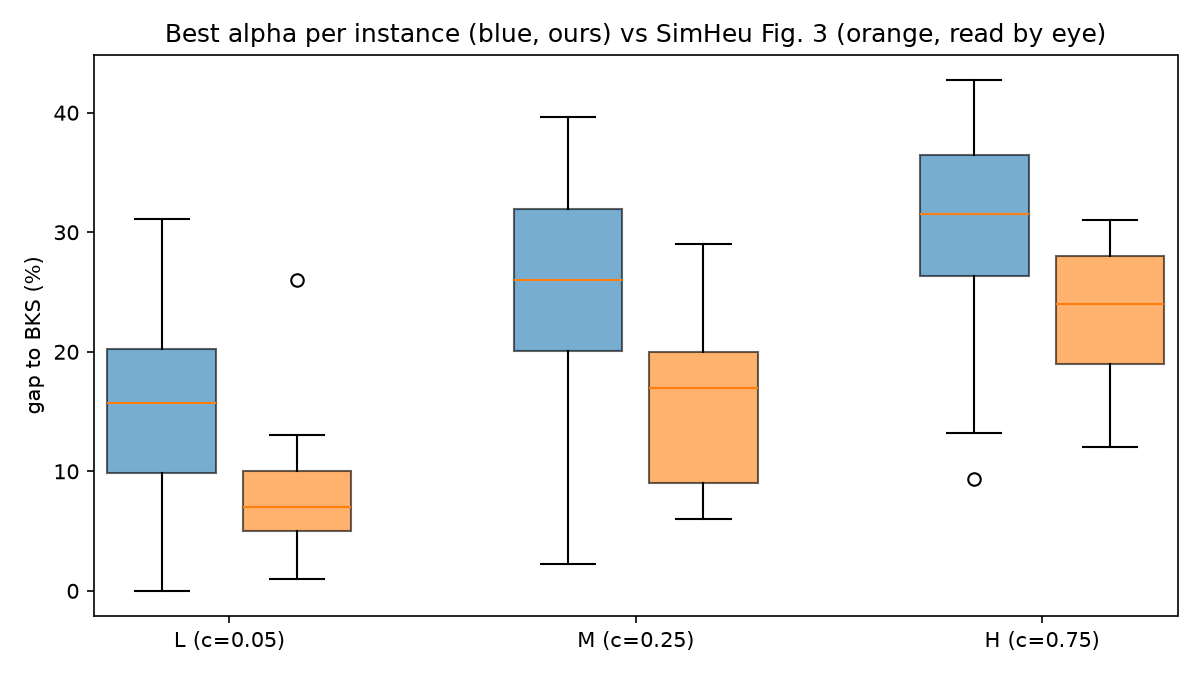
\includegraphics[width=0.85\textwidth]{gap_best_vs_paper.png}
\caption{Gap to the deterministic BKS per level, best $\alpha$ per instance. Blue: our 141 instances
(boxes Q1--Q3, line at the median, whiskers up to 1.5 IQR, circles beyond). Orange: SimHeu boxes of
Figure~3 of~\cite{juan2019}, read by eye.}
\label{fig:paper}
\end{figure}

\textbf{Comparison with the paper.} The gap grows with the uncertainty, L\,<\,M\,<\,H, as in the paper,
but our medians are 7--9 points higher (15.69, 26.02 and 31.56\,\% against about 7, 17 and 24\,\%), and
at L and M our lower quartile is about their upper one. The comparison is approximate: the values are
read by eye, and the paper says neither which instances enter each box (we assume p1--p3, the only sets
solved by the SAA) nor how the gap is computed. Our deterministic gap is only 2.4--3.2 points, so the
difference does not come mainly from the construction. A plausible cause is that Juan et al.\ simulate
inside the search loop and stop by time (their Figure~4 shows runs of up to about 400\,s), so simulation can steer the search towards
routes with slack, whereas we simulate only 7 candidates chosen with expected times; we cannot check it
without their code.

\textbf{Most of the gap is lost to uncertainty.} The median deterministic gap is zero at every
level: in 72, 72 and 82 of the 141 cases the winner reaches the BKS in deterministic terms. The
deterministic gap accounts for only 2.4--3.2 points and the loss due to uncertainty for 11.50, 22.06 and
28.10, about 80\,\% of the gap at L and 90\,\% at M and H. Measured on the winner's own reward, the loss
is 11.86, 22.72 and 28.79\,\%, almost the share of routes that arrive late on a simulated day (12.73, 23.57 and 29.45\,\%), as expected
when a late route loses everything. Part of it no solution can avoid. A likely reason for its size is
the one announced in Section~\ref{sec:method}: the median expected time of the winners' routes is
$0.93\,t_{\max}$ at every level, and 4, 6 and 8\,\% of them lie within 1\,\% of $t_{\max}$, where a route
fails almost half of the time. The simulation also often has little to choose from: in 27.1\,\% of the
1\,269 runs fewer than 7 distinct candidates survive, so the filter does not act, and in 9.0\,\% only one
does.

\textbf{The weight $\alpha$ hardly matters.} Over the 1\,269 runs the mean gap of each fixed $\alpha$
varies by less than 0.6 points within each level, and the best $\alpha$ is 0.25, 0.5 and 0.75 in 142, 138
and 143 cases. Yet keeping the best $\alpha$ per case lowers the mean gap by 1.3--2.2 points, partly
through the selection bias of picking the best of three with the reported mean.

\textbf{Set and $t_{\max}$.} Since short routes are relatively more variable, one would expect larger
gaps for small $t_{\max}$. The data show the opposite: the gap tends to grow with $t_{\max}$ (Spearman
0.49, 0.56 and 0.67 for L, M and H), and p2, with the smallest $t_{\max}$ (median 10.0 against 17.5 in p1
and 20.6 in p3), has the lowest gap. But the deterministic gap also grows with $t_{\max}$ (0.56, 0.54 and
0.59), more than the loss due to uncertainty (0.30, 0.39 and 0.44), and set and $t_{\max}$ are
confounded, since p2 has only 21 nodes: we report the trend as an observation, not an explanation.

\textbf{Time.} A run takes 0.053--0.234\,s (means 0.16--0.17\,s in p1 and p3, 0.07\,s in p2), and the 1\,269
runs about 25\,s on 12 threads. Figure~4 of~\cite{juan2019} reports a few seconds to about 400\,s in Java
on a 3.7\,GHz Xeon with a time limit, so only a qualitative comparison makes sense. Runs this cheap let
us try every $\alpha$ at every level instead of tuning one.

\section{Conclusions}

The simheuristic builds candidates for a deterministic world and lets Monte Carlo simulation, on
common days to rank and new days to measure, choose among them. On the 141 small Chao instances it
gives the ordering L\,<\,M\,<\,H of Juan et al., with mean gaps of $14.65$, $25.02$ and $30.51\,\%$, in a
fraction of a second per run. The winners usually match the BKS in deterministic terms, but the median
route fills $0.93\,t_{\max}$ and on average 13--29\,\% of the routes arrive late on a simulated day:
simulation can only choose among routes built without slack. The next step is a safety margin: building with $t_{\max}-\delta$ while simulating
with the true $t_{\max}$, with $\delta$ from a grid, from the route variance
($E_d+z\sqrt{c\,E_d}\le t_{\max}$) or adapted to the failure rate of the fast simulation.

\begin{thebibliography}{9}
\footnotesize\setlength{\itemsep}{0pt}\setlength{\parskip}{0pt}
\bibitem{juan2019} A.~A. Juan, L.~Reyes-Rubiano, R.~de la Torre, J.~Panadero, J.~Faulin and I.~Latorre.
Simulation-based optimization in transportation and logistics: comparing sample average approximation
with simheuristics. In \emph{Proc.\ 2019 Winter Simulation Conference}, 1906--1917, 2019.
\bibitem{chao1996} I.-M. Chao, B.~L. Golden and E.~A. Wasil. The team orienteering problem.
\emph{Eur.\ J.\ Oper.\ Res.}, 88(3):464--474, 1996.
\bibitem{panadero2021} J.~Panadero, M.~Ammouriova, A.~A. Juan, A.~Agustin, M.~Nogal and C.~Serrat.
Combining parallel computing and biased randomization for solving the team orienteering problem in
real-time. \emph{Appl.\ Sci.}, 11(24):12092, 2021.
\bibitem{grasas2017} A.~Grasas, A.~A. Juan, J.~Faulin, J.~de Armas and H.~Ramalhinho. Biased
randomization of heuristics using skewed probability distributions: a survey and some applications.
\emph{Comput.\ Ind.\ Eng.}, 110:216--228, 2017.
\bibitem{dang2013} D.-C. Dang, R.-N. Guibadj and A.~Moukrim. An effective PSO-inspired algorithm for the
team orienteering problem. \emph{Eur.\ J.\ Oper.\ Res.}, 229:332--344, 2013.
\end{thebibliography}

\end{document}
